% Gráfico de barras — Lote I (VSR e EF com IC 95% de Wilson, assimétrico)
% Requer pgfplots (já no preâmbulo). Rótulos de valor girados 90 graus.
\begin{figure}[htbp]
    \centering
    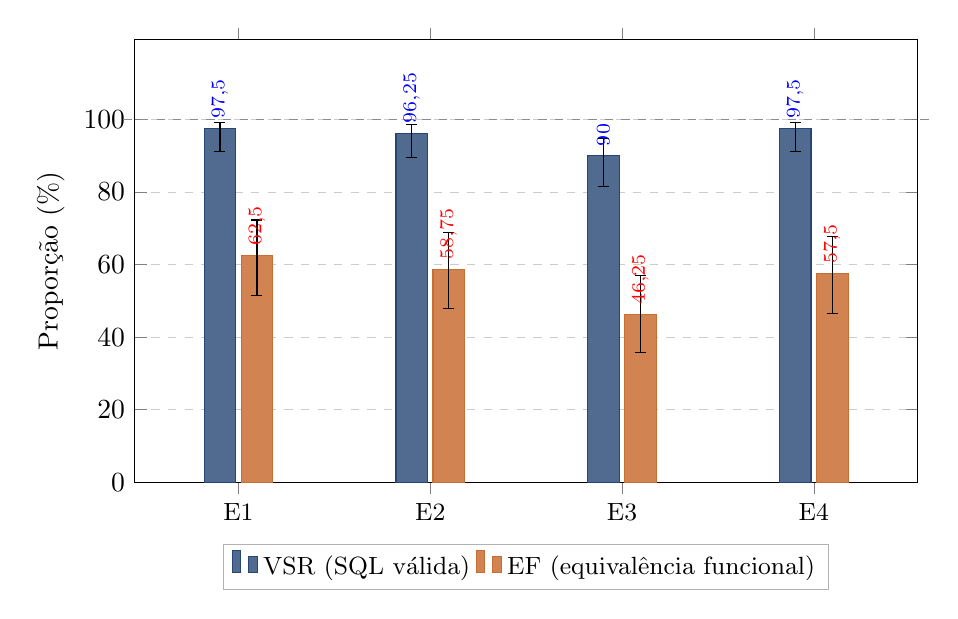
\begin{tikzpicture}
    \definecolor{simVSR}{RGB}{38,70,116}
    \definecolor{simEF}{RGB}{201,110,50}
    \begin{axis}[
        width=0.95\textwidth, height=7.2cm,
        ybar=2pt, bar width=0.40cm,
        ymin=0, ymax=122,
        ytick={0,20,40,60,80,100},
        ylabel={Proporção (\%)},
        xtick={1,2,3,4},
        xticklabels={E1, E2, E3, E4},
        xticklabel style={font=\small},
        enlarge x limits=0.18,
        ymajorgrids=true, grid style={dashed, black!20},
        legend style={at={(0.5,-0.14)}, anchor=north, legend columns=2,
                      draw=black!30, font=\small},
        nodes near coords,
        every node near coord/.append style={rotate=90, anchor=west, font=\scriptsize,
            /pgf/number format/.cd, use comma, fixed, precision=2},
        clip=false,
    ]
        % --- VSR (taxa de SQL válida) ---
        \addplot+[draw=simVSR, fill=simVSR!80,
            error bars/.cd, y dir=both, y explicit,
            error bar style={black, line width=0.5pt}]
          table[x=x, y=y, y error plus=ep, y error minus=em] {
            x   y       ep     em
            1   97.50   1.8    6.2
            2   96.25   2.45   6.75
            3   90.00   4.8    8.5
            4   97.50   1.8    6.2
          };
        \addlegendentry{VSR (SQL válida)}
        % --- EF (equivalência funcional) ---
        \addplot+[draw=simEF, fill=simEF!85,
            error bars/.cd, y dir=both, y explicit,
            error bar style={black, line width=0.5pt}]
          table[x=x, y=y, y error plus=ep, y error minus=em] {
            x   y       ep      em
            1   62.50   9.8     11.0
            2   58.75   10.15   10.95
            3   46.25   10.85   10.55
            4   57.50   10.2    10.9
          };
        \addlegendentry{EF (equivalência funcional)}
        % linha de referência em 100%
        \draw[black!45, dashed] (axis cs:0.4,100) -- (axis cs:4.6,100);
    \end{axis}
    \end{tikzpicture}
    \caption{Lote I --- VSR e EF por experimento ($n=80$; E1: GPT-4.1-mini com Prompt~A; E2: contexto estendido; E3: GPT-4o-mini; E4: GPT-4o). Barras de erro: IC 95\% (Wilson).}
    \label{fig:grafico_sql}
\end{figure}
